%
% File acl2016.tex
%
%% Based on the style files for ACL-2015, with some improvements
%%  taken from the NAACL-2016 style
%% Based on the style files for ACL-2014, which were, in turn,
%% Based on the style files for ACL-2013, which were, in turn,
%% Based on the style files for ACL-2012, which were, in turn,
%% based on the style files for ACL-2011, which were, in turn, 
%% based on the style files for ACL-2010, which were, in turn, 
%% based on the style files for ACL-IJCNLP-2009, which were, in turn,
%% based on the style files for EACL-2009 and IJCNLP-2008...

%% Based on the style files for EACL 2006 by 
%%e.agirre@ehu.es or Sergi.Balari@uab.es
%% and that of ACL 08 by Joakim Nivre and Noah Smith

\documentclass[11pt]{article}
\usepackage{acl2016}
\usepackage{times}
\usepackage{url}
\usepackage{latexsym}

% Required for images
\usepackage{graphicx}
\graphicspath{ {img/} }

\aclfinalcopy % Uncomment this line for the final submission
%\def\aclpaperid{***} %  Enter the acl Paper ID here

%\setlength\titlebox{5cm}
% You can expand the titlebox if you need extra space
% to show all the authors. Please do not make the titlebox
% smaller than 5cm (the original size); we will check this
% in the camera-ready version and ask you to change it back.

\newcommand\BibTeX{B{\sc ib}\TeX}

\title{Sentiment Analysis Stock Trading Via Twitter}

\author{
Jason Yao, Jenna Denker, James Zhang, Yu Li\\
Department of Computer Science,\\
Courant Institute of Mathematical Sciences\\
New York University,\\
New York, NY, USA\\
\{{\tt JasonYao, jld508, yjz208, yl2133}\}{\tt @nyu.edu}\\
\today
}
\date{\today}

\begin{document}
\maketitle
\begin{abstract}
The utilization of Sentiment Analysis (SA) on
Twitter tweets in our system has generated
profits of 1.8\% over a three week period in
April 2017. The market growth during that same
time period of the S\&P index was 0.02\%.
This performance increase was derived from
leveraging public sentiment about public
companies, which does factor into the stock
price of public companies. This paper will explore
the specific algorithm utilized to derive these
market gains, as well as future potential improvements
to improve profit yields over time.
\end{abstract}

\section{Introduction}
We use a custom built program built in Python 3,
leveraging Twitter's API in order to create an
automated trade file, which contains a list of
trades to be executed. Since the building of a
whole trading engine is wildly out of scope for
this analysis, we thus manually enter the generated
trades into a paper trading platform to show
the potential that SA has in regards to company
stock performance.

\section{Stocks Market Domain Knowledge}
\subsection{Call Options}
A {\bf call option} is an agreement between two investors that gives one the option, but not the obligation, to buy a stock of a company at a set price, known as the strike price within a certain time-frame.~\cite{call} Normally this occurs when an investor believes that a company's stock price will increase in the future, allowing the investor the ability to buy the stock at the current lower price, then sell the stock if the company's stock price has increased.

If, however, a company's stock value has decreased during this time, then there is no reason for the investor to buy at the strike price, when buying on the open market is cheaper. In this case, the investor will have lost the amount paid as a premium for the right to buy the stock at the strike price.

For example, if an investor bought a call option for 500 shares of IBM Stock with a strike price at \$100 when the share price is at \$90, set to expire in 2 months, the investor would theoretically pay \$5000 as their premium cost (\$10 x 500 shares). If the stock price increased to \$100, the investor will still be at a loss for \$5000 due to the premium cost. The investor will begin to make a profit when the IBM stock price exceeds \$110, when the \$10 gross profit covers the \$5000 premium cost.

\begin{figure}[h]
\centering
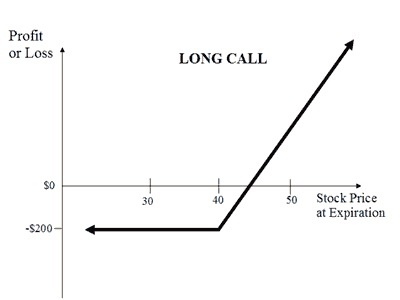
\includegraphics[scale=0.5]{long-call}
\caption{Example of a Call Option}
\end{figure}

\subsection{Put Options}
A {\bf put option} is an agreement between two investors that gives one the option, but not the obligation, to sell a stock of a company at a set price, known as the strike price within a certain time-frame.~\cite{put} Normally this occurs when an investor believes that a company's stock price will decrease in the future, allowing the investor the ability to sell the stock at the current higher price, and can be thought of as the opposite of a call option.

If, however, a company's stock value has increased during this time, then there is no reason for the investor to sell at the strike price. In this case, the investor will have lost the amount paid as a premium for the right to sell the stock at the strike price.

For example, if an investor bought a call option for 500 shares of IBM Stock with a strike price at \$100 when the share price is at \$90, set to expire in 2 months, the investor would theoretically pay \$5000 as their premium cost (\$10 x 500 shares). If the stock price increased to \$100, the investor will still be at a loss for \$5000 due to the premium cost. The investor will begin to make a profit when the IBM stock price exceeds \$110, when the \$10 gross profit covers the \$5000 premium cost.

For example, if an investor is bearish on UAL, which has a share price of \$75, the investor may put a put option for a period of 1 month for \$70 per share, plus a premium cost of \$1 per share. This means that in total, the investor has bought 500 shares and paid \$500 as a premium cost. If the stock price fell to \$70, then the investor would have still lost the \$500 premium cost. It's only if the stock price falls under to \$69, from which the investor begins to make a profit. On the other hand, if the stock price rose beyond \$70, the investor would let the option expire unexercised, and thus limiting the total cost to the investor to just the initial premium cost of \$500.

\begin{figure}[h]
\centering
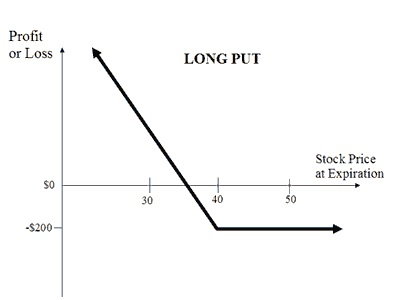
\includegraphics[scale=0.5]{long-put}
\caption{Example of a Put Option}
\end{figure}
    
\subsection{Strike Price}
The {\bf strike price} for an option is the fixed
amount at which an investor agrees to either buy
or sell an underlying asset such as a stock option.
For call options, the strike price is where the
security can be bought (up to the expiration date);
for put options, the strike price is the price at
which shares can be sold.~\cite{strike_price}

\begin{figure}[h]
\centering
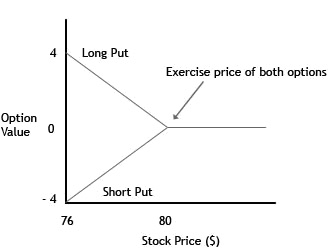
\includegraphics[scale=0.7]{strike-price}
\caption{Example of a Strike Price}
\end{figure}

\subsection{Algorithmic Strike Price Determination}
When manually entering trades into the paper
trading engine, the strike price was automatically
determined based off of the existing price, and a
simple percentage-based offset.

We divide each option into two categories: "Soft"
and "Hard". Soft options (soft calls and soft puts)
are generated in the trade file whenever the general
sentiment around a company affects its {\bf Viability Score}
(VS) to the point of passing the soft threshold, which
in our program was set to $\pm$ 200 VS. Likewise, hard
options (hard calls and hard puts) are generated in the
trade file whenever the general sentiment around a company
affects its VS to the point of passing the hard threshold,
which was set to $\pm$ 500 VS.

What this means is that if the general sentiment
surrounding a company becomes negative extremely
quickly, then the company's corresponding VS will
drop extremely quickly as well, allowing the program
to deduce from the general negative sentiment that
a negative public event has occurred (e.g. A PR fiasco,
or a bad earnings call), and to react to this event by
generating a hard put.

On the other hand, assuming that there's a general
positive sentiment trend for a company, its VS score
will gradually increase enough to the point where a soft
call will be generated instead.

\subsection{Stock Sentiment Bias}
In the stock market, the number of investors
who are willing to put money into stocks with
positive sentiment and outlook is much higher
than people who are willing to play on bad news.
This is likely due to the fact that the maximum
profit from a short is simply 100\% of a company's
stock value, which occurs extremely rarely.

On the other hand, however, there is no profit limit
for having long call positions, due to the potential
growth in value of the stock being unlimited in theory.
Thus it should be noted that a wave of positive
sentiment would likely drive the stock price of a
company up, while negative sentiment would not likely
drive the stock down as much. This means that the
overpricing of a stock's value is much more likely
than its underpricing in the market.

\section{System Overview}
The current system build is segregated
into two portions: the Ingestion Engine
and the Processing Engine. Due to it being
extremely out of scope for this project,
a Trading Engine was not built, though
one in theory could create one in order
to take the trade file generated by the
Processing Engine in order to automatically
place trades on a market, thus fully
automating the system.

\subsection{Ingestion Engine}
The Ingestion Engine is a simple
command-line wrapper that pulls Tweets
from Twitter via its Streaming API~\cite{streaming}.
Every 100 tweets are then batched together
for processing in the Processing Engine,
and future batches are queued up as required.

Due to the large amount of tweets being
ingested into the system itself, the general
amount of time required to process each batch
is close to 10 seconds. A way to mitigate this
required processing time would be to load-balance
incoming tweets, and spin up processing servers
as required to process and update company VS scores.

\subsection{Processing Engine}
The Processing Engine parses the given input
(tweets), combines it with historical data,
then computes and labels each given stock with
a Viability Score (VS). This score is calculated
from the given current sentiment about a stock,
and its current position in the marketplace, with
a higher differential resulting in a higher VS.

\section{Performance}
This algorithmic approach to stock trading
based off of Twitter users' sentiment analysis
derived gains of 1.8\%. In this same time
period, the S\&P index gained only a 0.02\%
increase, showing that it is at least possible
to generate a profit based off of the sentiment
analysis of Twitter users that can beat the
market in the short term.

In general, because of the deluge of tweets
coming into the system in real time, it is
not possible to process the tweets in a fast
enough manner using a single machine. However,
if the processing task was load-balanced with
multiple machines handling the processing of
information, it is then theoretically possible
to analyze the incoming tweets in real-time,
instead of having to batch and process tweets
in the current system.

\subsection{Viability Score}
The {\bf Viability Score} (VS) is a term used
to denote the "sentiment value" of a company
over time. As tweets stream into the system,
the VS of a given company will increase or
decrease to correspond with the general
sentiment around a company. When this sentiment
reaches a certain threshold, a trade will be
generated, and written into the trade file.
If a hard threshold is passed, the VS will
reset back to 0 to allow for further trades
to be conducted.

\section{Algorithm}
For each tweet, we do a first pass to extract
out any company names that can be found in the
tweet, based off of a pre-defined list of stock
tickers, full company names, and a selection of
colloquial names of companies.

After the first pass, assuming that at least one
company name was found, we then leverage the
Python library Textblob in order to gain the
sentiment analysis polarity and certainty of
the tweet.

The SA polarity is a floating point value
between -1 and 1, such that -1 corresponds
to an extremely low sentiment, while a value
of 1 corresponds to an extremely high sentiment.
An SA polarity score of 0 is neutral, and
thus does not truly affect the company in
question.

The SA certainty is a floating point value
between 0 and 1, such that 0 corresponds to
an extremely uncertain analysis, and 1 corresponds
to an extremely certain analysis. This is
useful in determining whether a tweet is truly
as positive or negative as its polarity value
would have us believe. High certainty scores
thus affects the VS generation much more than
low certainty scores.

After the SA polarity and certainty have
been extracted, the {\bf Viability Score} (VS)
is then generated from by the algorithm below:

$VS = VS_{old} + (SA_{polarity} * SA_{certainty} * \ln(impressions))$

\section{Future Improvements}
First and foremost, the biggest improvement to the
current system is the implementation of an automated
trading engine. In theory, the automated trading engine
would allow the system to run end-to-end, taking the
companies with high VS, and executing the trades immediately
in order to lessen the delay when it comes to having a
human investor manually execute the given trades in the
trade file.

Another potential improvement to further expand the existing
Ingestion Engine would be to implement monitoring of
trending hashtags on Twitter. Trending hashtags would
allow the system to more accurately monitor breaking
news and extreme cases which might not be caught as
fast by the user list currently implemented. These
extreme cases could include public relations disasters,
viral marketing campaigns, and even terrorist attacks,
each of which tend to have a large impact on the state
of the stock market, and the companies in them. Tweepy
has existing functionality to retrieve trending hashtags,
and the hashtags could be extracted alongside each batch
of tweets and processed accordingly.

Finally, another potential improvement to further expand the
capabilities of the system is to include the use of a neural
network in order to fine-tune thresholds to be company-specific.
Currently, all thresholds are globally applicable to all companies,
but it's easy to see situations in which this is not acceptable.
Highly popular companies such as Tesla or Facebook are talked about
much more frequently than others, and having rarely-talked about
companies explode in sentiment value should generate a higher VS,
and have lower thresholds due to their rare use. This would also
have the benefit of lessening false positives, and would allow the
system to better understand whether a trade is a good choice based
off of historical, financial, and sentiment data, along with any
extruding market factor at the time of the trade.

\section{Conclusion}
By analyzing the sentiment around Twitter users,
it is possible to generate a "sentiment value" score
about publicly traded companies, and to then use these
trades in order to generate a profit that could beat
the market in the short term. The current paper profit
yield of 1.8\% while the S\&P index had a growth
of 0.02\% showcases the ability to leverage sentiment
analysis in the pursuit of intra-day profits.

\newpage
\section{References}
\bibliography{acl2016}{}
\bibliographystyle{acl2016}


\end{document}
